\section{永磁同步电机的数学模型}
\subsection{基本数学方程\label{sec:基本数学方程}}
永磁同步电机通过给三相定子回路施加特定的电压，使得定子构造出旋转磁场，
带动转子旋转。并且定义永磁体磁矩方向与电机A相的夹角为电角度\(\theta_{\mathrm{e}}\)。
\begin{figure}[H]
    \begin{minipage}{0.5\textwidth}
        \centering
        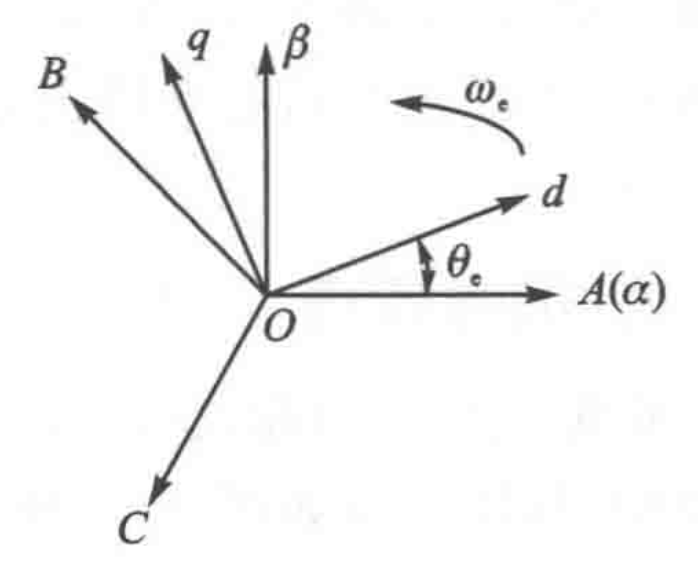
\includegraphics[width=\textwidth]{图片/三种坐标关系图.png}
        \caption{三种坐标关系图}
    \end{minipage}
    \begin{minipage}{0.5\textwidth}
        \centering
        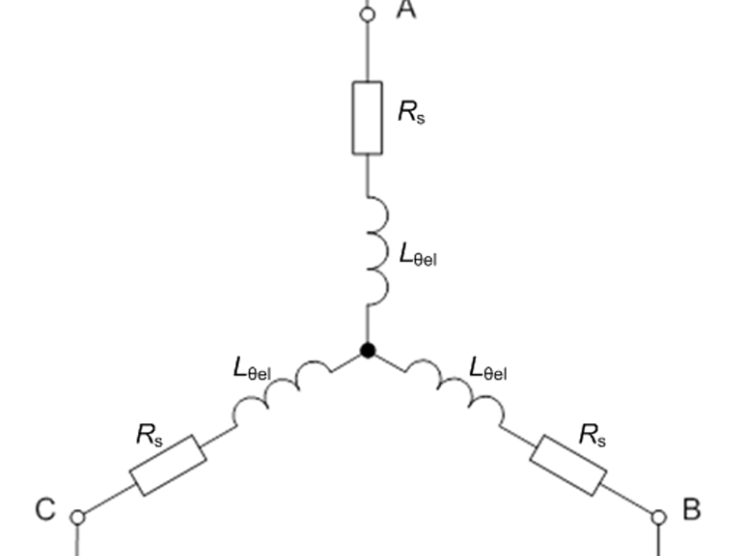
\includegraphics[width=\textwidth]{图片/三相电机电路图.PNG}
        \caption{三相电机电路图}
    \end{minipage}
\end{figure}

根据永磁体的嵌入位置，可以将永磁同步电机（PMSM）分为表贴式永磁同步电机（SPMSM）和内置式永磁同步电机（IPMSM）。
表贴式永磁同步电机是指永磁体嵌入在转子的表面，磁路对称，属于隐极电机。
而内置式永磁同步电机是指永磁体嵌入在转子的内部，磁路不对称，属于凸极电机。

接下来，讨论自然坐标系A-B-C下的永磁同步电机数学模型。对于每一相的电压、电流，
考虑存在相电阻\(R\)和相电感\(L\)。根据基尔霍夫电流定律，有\(i_{\mathrm{A}}+i_{\mathrm{B}}+i_{\mathrm{C}}=0\)。
以A相为例，在不考虑耦合时根据基尔霍夫电压定律可得
\begin{equation*}
    u_{\mathrm{A}}=R_{\mathrm{A}}i_{\mathrm{A}}+L_{\mathrm{A}}\cfrac{\dd}{\dd t}i_{\mathrm{A}}
\end{equation*}

考虑到电感之间的互感效应，会存在B、C相电感对A相电压的影响，也就有
\begin{equation*}
    u_{\mathrm{A}}=R_{\mathrm{A}}i_{\mathrm{A}}+L_{\mathrm{A}}\cfrac{\dd}{\dd t}i_{\mathrm{A}}+M_{\mathrm{BA}}\cfrac{\dd}{\dd t}i_{\mathrm{B}}+M_{\mathrm{CA}}\cfrac{\dd}{\dd t}i_{\mathrm{C}}
\end{equation*}

除此之外，转子的永磁体磁场也会对A相电感磁场造成影响。若永磁体磁链为\(\psi_{\mathrm{m}}\)，那么
永磁体磁链在三相上的分量为
\begin{equation*}
    \begin{cases}
        \psi_{\mathrm{A}}=\psi_{\mathrm{m}}\cos\theta_{\mathrm{e}}\\
        \psi_{\mathrm{B}}=-\psi_{\mathrm{m}}\cos(\cfrac{\pi}{3}+\theta_{\mathrm{e}})=
        \psi_{\mathrm{m}}\cos(\theta_{\mathrm{e}}-\cfrac{2\pi}{3})\\
        \psi_{\mathrm{C}}=-\psi_{\mathrm{m}}\cos(\cfrac{\pi}{3}-\theta_{\mathrm{e}})=
        \psi_{\mathrm{m}}\cos(\theta_{\mathrm{e}}+\cfrac{2\pi}{3})
    \end{cases}
\end{equation*}

因此完整的三相电路方程为
\begin{equation*}
    \begin{cases}
        u_{\mathrm{A}}=R_{\mathrm{A}}i_{\mathrm{A}}+L_{\mathrm{A}}\cfrac{\dd}{\dd t}i_{\mathrm{A}}+M_{\mathrm{BA}}\cfrac{\dd}{\dd t}i_{\mathrm{B}}+M_{\mathrm{CA}}
        \cfrac{\dd}{\dd t}i_{\mathrm{C}}+\cfrac{\dd}{\dd t}\psi_{\mathrm{A}}\\
        u_{\mathrm{B}}=R_{\mathrm{B}}i_{\mathrm{B}}+L_{\mathrm{B}}\cfrac{\dd}{\dd t}i_{\mathrm{B}}+M_{\mathrm{AB}}\cfrac{\dd}{\dd t}i_{\mathrm{A}}+M_{\mathrm{CB}}
        \cfrac{\dd}{\dd t}i_{\mathrm{C}}+\cfrac{\dd}{\dd t}\psi_{\mathrm{B}}\\
        u_{\mathrm{C}}=R_{\mathrm{C}}i_{\mathrm{C}}+L_{\mathrm{C}}\cfrac{\dd}{\dd t}i_{\mathrm{C}}+M_{\mathrm{AC}}\cfrac{\dd}{\dd t}i_{\mathrm{A}}+M_{\mathrm{BC}}
        \cfrac{\dd}{\dd t}i_{\mathrm{C}}+\cfrac{\dd}{\dd t}\psi_{\mathrm{C}}
    \end{cases}
\end{equation*}

用矩阵形式表示为
\begin{equation*}
    \begin{bmatrix}
        u_{\mathrm{A}}\\u_{\mathrm{B}}\\u_{\mathrm{C}}
    \end{bmatrix}
    =
    \begin{bmatrix}
        R_{\mathrm{A}}&0&0\\0&R_{\mathrm{B}}&0\\0&0&R_{\mathrm{C}}
    \end{bmatrix}
    \begin{bmatrix}
        i_{\mathrm{A}}\\i_{\mathrm{B}}\\i_{\mathrm{C}}
    \end{bmatrix}
    +
    \begin{bmatrix}
        L_{\mathrm{A}}&M_{\mathrm{BA}}&M_{\mathrm{CA}}\\
        M_{\mathrm{AB}}&L_{\mathrm{B}}&M_{\mathrm{CB}}\\
        M_{\mathrm{AC}}&M_{\mathrm{BC}}&L_{\mathrm{C}}
    \end{bmatrix}
    \begin{bmatrix}
        \cfrac{\dd}{\dd t}i_{\mathrm{A}}\\
        \cfrac{\dd}{\dd t}i_{\mathrm{B}}\\
        \cfrac{\dd}{\dd t}i_{\mathrm{C}}
    \end{bmatrix}
    -
    \psi_{\mathrm{m}}\omega_{\mathrm{e}}
    \begin{bmatrix}
        \sin\theta_{\mathrm{e}}\\
        \sin(\theta_{\mathrm{e}}-\cfrac{2\pi}{3})\\
        \sin(\theta_{\mathrm{e}}+\cfrac{2\pi}{3})
    \end{bmatrix}
\end{equation*}

需要注意的是，若永磁同步电机为凸极电机（IPMSM），那么电感（包括自感和互感）
不是常数，其值会随着电角度而发生变化。自感值和互感值可以用下式表示。存在电角度的二次谐波，其主要原因是
对于定子而言，不对称的椭圆磁路每转过180°电角度，永磁体对其的影响就发生一个周期的变化。
\begin{minipage}{0.5\textwidth}
    \begin{equation*}
        \begin{cases}
            L_{\mathrm{A}}=L_{\mathrm{A}0}-L_{\mathrm{A}2}\cos2\theta_{\mathrm{e}}\\
            L_{\mathrm{B}}=L_{\mathrm{B}0}-L_{\mathrm{B}2}\cos(2\theta_{\mathrm{e}}-\cfrac{4\pi}{3})\\
            L_{\mathrm{C}}=L_{\mathrm{C}0}-L_{\mathrm{C}2}\cos(2\theta_{\mathrm{e}}+\cfrac{4\pi}{3})
        \end{cases}
    \end{equation*}
\end{minipage}
\begin{minipage}{0.5\textwidth}
    \begin{equation*}
        \begin{cases}
            M_{\mathrm{AB}}=M_{\mathrm{BA}}=M_{\mathrm{AB}0}-M_{\mathrm{AB}2}\cos(2\theta_{\mathrm{e}}+\cfrac{4\pi}{3})\\
            M_{\mathrm{BC}}=M_{\mathrm{CB}}=M_{\mathrm{BC}0}-M_{\mathrm{BC}2}\cos2\theta_{\mathrm{e}}\\
            M_{\mathrm{AC}}=M_{\mathrm{CA}}=M_{\mathrm{AC}0}-M_{\mathrm{AC}2}\cos(2\theta_{\mathrm{e}}-\cfrac{4\pi}{3})
        \end{cases}
    \end{equation*}
\end{minipage}

理想情况下电机为三相对称电路，即有
\(\begin{cases}
    R_{\mathrm{A}}=R_{\mathrm{B}}=R_{\mathrm{C}}=R_{\mathrm{s}}\\
    L_{\mathrm{A}0}=L_{\mathrm{B}0}=L_{\mathrm{C}0}=L_{\mathrm{s}0}\\
    L_{\mathrm{A}2}=L_{\mathrm{B}2}=L_{\mathrm{C}2}=L_{\mathrm{s}2}\\
    M_{\mathrm{AB}0}=M_{\mathrm{BC}0}=M_{\mathrm{AC}0}=M_{\mathrm{s}0}\\
    M_{\mathrm{AB}2}=M_{\mathrm{BC}2}=M_{\mathrm{AC}2}=M_{\mathrm{s}2}
\end{cases}\)，

那么电路方程可以简化表示为
\begin{equation*}
    \begin{bmatrix}
        u_{\mathrm{A}}\\u_{\mathrm{B}}\\u_{\mathrm{C}}
    \end{bmatrix}
    =
    R_{\mathrm{s}}
    \begin{bmatrix}
        i_{\mathrm{A}}\\i_{\mathrm{B}}\\i_{\mathrm{C}}
    \end{bmatrix}
    +
    \cfrac{\dd}{\dd t}
    \Big(\bm{L}(\theta_{\mathrm{e}})
    \begin{bmatrix}
        i_{\mathrm{A}}\\i_{\mathrm{B}}\\i_{\mathrm{C}}
    \end{bmatrix}
    \Big)-
    \psi_{\mathrm{m}}\omega_{\mathrm{e}}
    \begin{bmatrix}
        \sin\theta_{\mathrm{e}}\\
        \sin(\theta_{\mathrm{e}}-\cfrac{2\pi}{3})\\
        \sin(\theta_{\mathrm{e}}+\cfrac{2\pi}{3})
    \end{bmatrix}
\end{equation*}

对微分项展开可得
\(\cfrac{\dd}{\dd t}\Big(\bm{L}(\theta_{\mathrm{e}})
\begin{bmatrix}
    {{i_{\mathrm{A}}}}\\{{i_{\mathrm{B}}}}\\{{i_{\mathrm{C}}}}
\end{bmatrix}\Big)
=
\cfrac{\dd}{\dd t}\bm{L}(\theta_{\mathrm{e}})
\begin{bmatrix}
    i_{\mathrm{A}}\\i_{\mathrm{B}}\\i_{\mathrm{C}}
\end{bmatrix}
+
\bm{L}(\theta_{\mathrm{e}})
\begin{bmatrix}
    \dot{i_{\mathrm{A}}}\\\dot{i_{\mathrm{B}}}\\\dot{i_{\mathrm{C}}}
\end{bmatrix}\)
\footnote{\(\dot{x}\)表示对信号\(x\)进行时间微分，即
\(\dot{x}=\cfrac{\dd x}{\dd t}\)}

电感矩阵微分为
\begin{equation}
    \cfrac{\dd}{\dd t}\bm{L}(\theta_{\mathrm{e}})
    =2\omega_{\mathrm{e}}
    \begin{bmatrix}
        L_{\mathrm{s}2}\sin2\theta_{\mathrm{e}}
        &M_{\mathrm{s}2}\sin(2\theta_{\mathrm{e}}+\cfrac{4\pi}{3})
        &M_{\mathrm{s}2}\sin(2\theta_{\mathrm{e}}-\cfrac{4\pi}{3})
        \\
        M_{\mathrm{s}2}\sin(2\theta_{\mathrm{e}}+\cfrac{4\pi}{3})
        &L_{\mathrm{s}2}\sin(2\theta_{\mathrm{e}}-\cfrac{4\pi}{3})
        &M_{\mathrm{s}2}\sin2\theta_{\mathrm{e}}
        \\
        M_{\mathrm{s}2}\sin(2\theta_{\mathrm{e}}-\cfrac{4\pi}{3})
        &M_{\mathrm{s}2}\sin2\theta_{\mathrm{e}}
        &L_{\mathrm{s}2}\sin(2\theta_{\mathrm{e}}+\cfrac{4\pi}{3})
    \end{bmatrix}
    \label{eq:电感矩阵微分}
\end{equation}

因此完整的电路表达式如下式表示：
\begin{align*}
    \begin{bmatrix}
        u_{\mathrm{A}} \\ u_{\mathrm{B}} \\ u_{\mathrm{C}}
    \end{bmatrix} &=
    \begin{bmatrix}
        2\omega_{\mathrm{e}}L_{\mathrm{s}2}\sin2\theta_{\mathrm{e}}+R_{\mathrm{s}}
        & 2\omega_{\mathrm{e}}M_{\mathrm{s}2}\sin(2\theta_{\mathrm{e}}+\cfrac{4\pi}{3})
        & 2\omega_{\mathrm{e}}M_{\mathrm{s}2}\sin(2\theta_{\mathrm{e}}-\cfrac{4\pi}{3})
        \\
        2\omega_{\mathrm{e}}M_{\mathrm{s}2}\sin(2\theta_{\mathrm{e}}+\cfrac{4\pi}{3})
        & 2\omega_{\mathrm{e}}L_{\mathrm{s}2}\sin2(\theta_{\mathrm{e}}-\cfrac{4\pi}{3})+R_{\mathrm{s}}
        & 2\omega_{\mathrm{e}}M_{\mathrm{s}2}\sin2\theta_{\mathrm{e}}
        \\
        2\omega_{\mathrm{e}}M_{\mathrm{s}2}\sin(2\theta_{\mathrm{e}}-\cfrac{4\pi}{3})
        & 2\omega_{\mathrm{e}}M_{\mathrm{s}2}\sin2\theta_{\mathrm{e}}
        & 2\omega_{\mathrm{e}}L_{\mathrm{s}2}\sin(2\theta_{\mathrm{e}}+\cfrac{4\pi}{3})+R_{\mathrm{s}}
    \end{bmatrix}
    \begin{bmatrix}
        i_{\mathrm{A}} \\ i_{\mathrm{B}} \\ i_{\mathrm{C}}
    \end{bmatrix} \\
    & +
    \begin{bmatrix}
        L_{\mathrm{s}0}-L_{\mathrm{s}2}\cos2\theta_{\mathrm{e}}
        & M_{\mathrm{s}0}-M_{\mathrm{s}2}\cos(2\theta_{\mathrm{e}}+\cfrac{4\pi}{3})
        & M_{\mathrm{s}0}-M_{\mathrm{s}2}\cos(2\theta_{\mathrm{e}}-\cfrac{4\pi}{3})
        \\
        M_{\mathrm{s}0}-M_{\mathrm{s}2}\cos(2\theta_{\mathrm{e}}+\cfrac{4\pi}{3})
        & L_{\mathrm{s}0}-L_{\mathrm{s}2}\cos(2\theta_{\mathrm{e}}-\cfrac{4\pi}{3})
        & M_{\mathrm{s}0}-M_{\mathrm{s}2}\cos2\theta_{\mathrm{e}}
        \\
        M_{\mathrm{s}0}-M_{\mathrm{s}2}\cos(2\theta_{\mathrm{e}}-\cfrac{4\pi}{3})
        & M_{\mathrm{s}0}-M_{\mathrm{s}2}\cos2\theta_{\mathrm{e}}
        & L_{\mathrm{s}0}-L_{\mathrm{s}2}\cos(2\theta_{\mathrm{e}}+\cfrac{4\pi}{3})
    \end{bmatrix}
    \begin{bmatrix}
        \dot{i_{\mathrm{A}}} \\ \dot{i_{\mathrm{B}}} \\ \dot{i_{\mathrm{C}}}
    \end{bmatrix} \\
    & -
    \psi_{\mathrm{m}}\omega_{\mathrm{e}}
    \begin{bmatrix}
        \sin\theta_{\mathrm{e}} \\
        \sin(\theta_{\mathrm{e}}-\cfrac{2\pi}{3}) \\
        \sin(\theta_{\mathrm{e}}+\cfrac{2\pi}{3})
    \end{bmatrix}
\end{align*}

为了简化表示，定义向量
\(
\bm{U}_{\mathrm{ABC}}=
\begin{bmatrix}
    u_{\mathrm{A}}\\u_{\mathrm{B}}\\u_{\mathrm{C}}
\end{bmatrix},
\bm{I}_{\mathrm{ABC}}=
\begin{bmatrix}
    i_{\mathrm{A}}\\i_{\mathrm{B}}\\i_{\mathrm{C}}
\end{bmatrix},
\bm{L}_{\mathrm{ABC}}=
\bm{L}(\theta),
\bm{\varPsi}_{\mathrm{ABC}}=
\begin{bmatrix}
    \psi_{\mathrm{A}}\\\psi_{\mathrm{B}}\\\psi_{\mathrm{C}}
\end{bmatrix}
=\psi_{\mathrm{m}}
\begin{bmatrix}\cos\theta_{\mathrm{e}}\\
    \cos(\theta_{\mathrm{e}}-\cfrac{2\pi}{3})\\
    \cos(\theta_{\mathrm{e}}+\cfrac{2\pi}{3})
\end{bmatrix}
\)
那么电路方程可以表示为
\begin{equation}
    \bm{U}_{\mathrm{ABC}}=
    R_{\mathrm{s}}\bm{I}_{\mathrm{ABC}}+
    {\dot{\bm{L}}_{\mathrm{ABC}}\bm{I}_{\mathrm{ABC}}+
    \bm{L}_{\mathrm{ABC}}\dot{\bm{I}}_{\mathrm{ABC}}}
    +{\dot{\bm{\varPsi}}_{\mathrm{ABC}}}
    \label{eq:自然坐标系电路方程}
\end{equation}

接下来讨论自然坐标系下永磁同步电机的电磁转矩表达式，这是连接电路和机械运动的关
键方程。首先，机械角度\(\theta_{\mathrm{m}}\)、机械角速度\(\omega_{\mathrm{m}}\)、
电角度\(\theta_{\mathrm{e}}\)、电角速度与电机的磁极对数\(p\)满足    
\(p\omega_{\mathrm{m}}=\omega_{\mathrm{e}},p\theta_{\mathrm{m}}=\theta_{\mathrm{e}}\)。

从能量守恒角度分析，电机中的功率总表达式为
\(P_{\mathrm{in}}=P_{\mathrm{Cu}}+\cfrac{\dd W_{\mathrm{m}}}{\dd t}+P_{\mathrm{e}}\)
。其中\(P_{\mathrm{in}}\)表示输入功率，\(P_{\mathrm{Cu}}\)表示定子铜损，
\(\cfrac{\dd W_{\mathrm{m}}}{\dd t}\)表示维持磁场的无功功率
，\(P_{\mathrm{e}}\)表示电磁功率。也就是说电磁功率可以表示为
\(P_{\mathrm{e}}=P_{\mathrm{in}}-P_{\mathrm{Cu}}-\cfrac{\dd W_{\mathrm{m}}}{\dd t}\)

定子铜损即相电阻上消耗的电功率，计算式为\(P_{\mathrm{Cu}}=R_{\mathrm{s}}(i_{\mathrm{A}}^2+i_{\mathrm{B}}^2+i_{\mathrm{C}}^2)\)
用矩阵表示为
\begin{equation*}
    P_{\mathrm{Cu}}=R_{\mathrm{s}}\bm{I}^T_{\mathrm{ABC}}\bm{I}_{\mathrm{ABC}}
\end{equation*}

电磁功率即输出的功率，和电磁转矩与机械角速度满足
\begin{equation*}
    P_{\mathrm{e}}=T_{\mathrm{e}}\omega_{\mathrm{m}}
\end{equation*}

无功功率主要用于维持磁场。根据磁场能表达式\(W_{\mathrm{m}}=\cfrac 12 LI^2\)，因此无功功率有：
\begin{equation*}
    \cfrac{\dd W_{\mathrm{m}}}{\dd t}=\cfrac 12
\cfrac{\dd}{\dd t}\bm{I}^T_{\mathrm{ABC}}\bm{L}_{\mathrm{ABC}}\bm{I}_{\mathrm{ABC}}
\end{equation*}

根据微分链式法则可以展开为三项之和：
\begin{equation*}
    \cfrac{\dd W_{\mathrm{m}}}{\dd t}=
\cfrac 12
(\dot{\bm{I}}^T_{\mathrm{ABC}}\bm{L}_{\mathrm{ABC}}\bm{I}_{\mathrm{ABC}}+
\bm{I}^T_{\mathrm{ABC}}\dot{\bm{L}}_{\mathrm{ABC}}\bm{I}_{\mathrm{ABC}}+
\bm{I}^T_{\mathrm{ABC}}\bm{L}_{\mathrm{ABC}}\dot{\bm{I}}_{\mathrm{ABC}})
\end{equation*}

由于\(\bm{L}_{\mathrm{ABC}}\)为对称矩阵，
因此\(\dot{\bm{I}}^T_{\mathrm{ABC}}\bm{L}_{\mathrm{ABC}}\bm{I}_{\mathrm{ABC}}
=\bm{I}^T_{\mathrm{ABC}}\bm{L}_{\mathrm{ABC}}\dot{\bm{I}}_{\mathrm{ABC}}\)
也就可得
\begin{equation*}
    \cfrac{\dd W_{\mathrm{m}}}{\dd t}=
\dot{\bm{I}}^T_{\mathrm{ABC}}\bm{L}_{\mathrm{ABC}}\bm{I}_{\mathrm{ABC}}+
\cfrac 12\bm{I}^T_{\mathrm{ABC}}\dot{\bm{L}}_{\mathrm{ABC}}\bm{I}_{\mathrm{ABC}}
\end{equation*}

电机的输入功率表达式为\(P_{\mathrm{in}}=\bm{U}_{\mathrm{ABC}}^T\bm{I}_{\mathrm{ABC}}\)
展开得到：
\begin{equation*}
    P=R_{\mathrm{s}}\bm{I}^T_{\mathrm{ABC}}\bm{I}_{\mathrm{ABC}}+\bm{I}^T_{\mathrm{ABC}}
\dot{\bm{L}}^T_{\mathrm{ABC}}\bm{I}_{\mathrm{ABC}}+\dot{\bm{I}}^T_{\mathrm{ABC}}
\bm{L}^T_{\mathrm{ABC}}\bm{I}_{\mathrm{ABC}}+\dot{\bm{\varPsi}}^T_{\mathrm{ABC}}\bm{I}_{\mathrm{ABC}}
\end{equation*}

由于电感矩阵为对称矩阵，因此可以表示为
\begin{equation*}
    P=R_{\mathrm{s}}\bm{I}^T_{\mathrm{ABC}}\bm{I}_{\mathrm{ABC}}+
    \bm{I}^T_{\mathrm{ABC}}\dot{\bm{L}}_{\mathrm{ABC}}\bm{I}_{\mathrm{ABC}}+
    {\bm{I}}^T_{\mathrm{ABC}}\bm{L}_{\mathrm{ABC}}\bm{I}_{\mathrm{ABC}}+
    \dot{\bm{\varPsi}}^T_{\mathrm{ABC}}\bm{I}_{\mathrm{ABC}}  
\end{equation*}

根据输入功率表达式可知：
\begin{equation*}
    P_{\mathrm{e}}=P-R_{\mathrm{s}}\bm{I}^T_{\mathrm{ABC}}\bm{I}_{\mathrm{ABC}}-
(\dot{\bm{I}}^T_{\mathrm{ABC}}\bm{L}_{\mathrm{ABC}}\bm{I}_{\mathrm{ABC}}
+\cfrac 12\bm{I}^T_{\mathrm{ABC}}\dot{\bm{L}}_{\mathrm{ABC}}\bm{I}_{\mathrm{ABC}})
\end{equation*}

可得电磁功率表达式为：
\begin{equation*}
    P_{\mathrm{e}}=\cfrac 12\bm{I}^T_{\mathrm{ABC}}\dot{\bm{L}}_{\mathrm{ABC}}
\bm{I}_{\mathrm{ABC}}+\dot{\bm{\varPsi}}^T_{\mathrm{ABC}}\bm{I}_{\mathrm{ABC}}
\end{equation*}

两边除以机械角速度即可得到电磁转矩表达式
\begin{equation}
    T_{\mathrm{e}}=\cfrac{1}{\omega_{\mathrm{m}}}
    (\cfrac 12\bm{I}^T_{\mathrm{ABC}}\dot{\bm{L}}_{\mathrm{ABC}}\bm{I}_{\mathrm{ABC}}
    +\dot{\bm{\varPsi}}^T_{\mathrm{ABC}}\bm{I}_{\mathrm{ABC}})
    \label{eq:自然坐标系电磁转矩表达式}
\end{equation}

\subsection{克拉克变换与帕克变换}
根据\ref{sec:基本数学方程}中的推导可知，在A-B-C三相自然坐标系下描述永磁同步电机的行为是非常复杂的。
因此更常采用坐标变换的方法，将三相自然坐标系转换为更方便描述的同步旋转坐标系。
这一过程需要通过克拉克变换和帕克变换两个步骤。

克拉克变换旨在将A-B-C三相自然坐标系转换为正交基底的两相静止坐标系\(\alpha-\beta\)，
。两个坐标系的关系如下图所示
\begin{figure}[H]
    \centering
    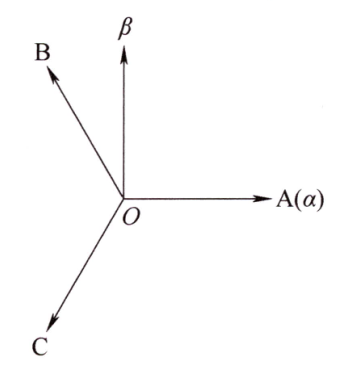
\includegraphics[width=0.4\textwidth]
    {图片/克拉克变换.png}
    \caption{克拉克变换}
\end{figure}

根据线性变换的知识，三相自然坐标系下的三个相差120°的单位向量，在两相静止坐标系下
可以表示为
\(
\begin{bmatrix}
    1&-\cfrac12&-\cfrac12\\
    0&\cfrac{\sqrt{3}}{2}&-\cfrac{\sqrt{3}}{2}
\end{bmatrix}
\)
，为了便于后续的计算，会进行等幅值变换，即希望变换前后满足\(i_{\mathrm{A}}=i_{\mathrm{\alpha}}\)，也就是
确定常数\(k\)使得
\(
k
\begin{bmatrix}
    1&-\cfrac12&-\cfrac12\\
    0&\cfrac{\sqrt{3}}{2}&-\cfrac{\sqrt{3}}{2}
\end{bmatrix}
\begin{bmatrix}
    1\\-\cfrac 12\\-\cfrac 12
\end{bmatrix}
=\begin{bmatrix}1\\0\end{bmatrix}
\)
，可以解得\(k=\cfrac 23\)。

此外，三相自然坐标系是三维的，而两相静止坐标系是二维的。为了方便矩阵求逆，也为了
描述三相电机的电流制约关系，会加入零序分量\(i_{\mathrm{0}}=\cfrac{1}{3}(i_{\mathrm{A}}+i_{\mathrm{B}}+i_{\mathrm{C}})=0\)。

最终得到克拉克变换公式
\begin{equation}
    \begin{bmatrix}
        i_{\mathrm{\alpha}}\\i_{\mathrm{\beta}}\\i_{\mathrm{0}}
    \end{bmatrix}
    =\cfrac 23
    \begin{bmatrix}
        1&-\cfrac12&-\cfrac12
        \\0&\cfrac{\sqrt{3}}{2}&-\cfrac{\sqrt{3}}{2}\\
        \cfrac{1}{2}&\cfrac{1}{2}&\cfrac{1}{2}
    \end{bmatrix}
    \begin{bmatrix}
        i_{\mathrm{A}}\\i_{\mathrm{B}}\\i_{\mathrm{C}}
    \end{bmatrix}
    \label{eq:克拉克变换}
\end{equation}

对于矩阵求逆可得克拉克逆变换公式
\begin{equation}
    \begin{bmatrix}
        i_{\mathrm{A}}\\i_{\mathrm{B}}\\i_{\mathrm{C}}
    \end{bmatrix}
    =\begin{bmatrix}
        1&0&1
        \\-\cfrac 12&\cfrac{\sqrt{3}}{2}&1
        \\-\cfrac 12&-\cfrac{\sqrt{3}}{2}&1
    \end{bmatrix}
    \begin{bmatrix}
        i_{\mathrm{\alpha}}\\i_{\mathrm{\beta}}\\i_{\mathrm{0}}
    \end{bmatrix}
    \label{eq:克拉克逆变换}
\end{equation}

接下来需要进行帕克变换，实现从两相静止坐标系到同步旋转坐标系的变换。定义沿着永磁
体旋转方向，与永磁体磁链同方向的轴为直轴d/D，超前直轴90°为交轴q/Q。d轴与
\(\mathrm{A(\alpha)}\)的夹角就是电角度\(\theta_{\mathrm{e}}\)
\begin{figure}[H]
    \centering
    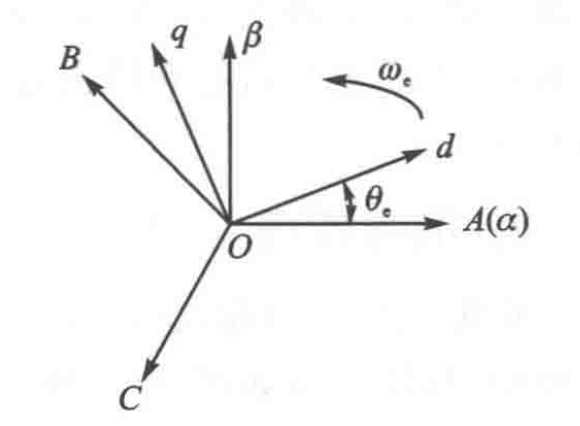
\includegraphics[width=0.4\textwidth]
    {图片/帕克变换.png}
    \caption{帕克变换}
\end{figure}

两相静止坐标系在的单位矢量在同步旋转坐标系下表示为
\(
\begin{bmatrix}
    \cos\theta_{\mathrm{e}}&\sin\theta_{\mathrm{e}}\\-\sin\theta_{\mathrm{e}}&\cos\theta_{\mathrm{e}}
\end{bmatrix}\)
可得帕克变换公式为
\begin{equation}
    \begin{bmatrix}
        i_{\mathrm{d}}\\i_{\mathrm{q}}\\i_{\mathrm{0}}
    \end{bmatrix}
    =
    \begin{bmatrix}
        \cos\theta_{\mathrm{e}}&\sin\theta_{\mathrm{e}}&0
        \\-\sin\theta_{\mathrm{e}}&\cos\theta_{\mathrm{e}}&0
        \\0&0&1
    \end{bmatrix}
    \begin{bmatrix}
        i_{\mathrm{\alpha}}
            \\i_{\mathrm{\beta}}
            \\i_{\mathrm{0}}
    \end{bmatrix}
    \label{eq:帕克变换}
\end{equation}

而帕克逆变换公式为
\begin{equation}
    \begin{bmatrix}
        i_{\mathrm{\alpha}}\\i_{\mathrm{\beta}}\\i_{\mathrm{0}}
    \end{bmatrix}
    =
    \begin{bmatrix}
        \cos\theta_{\mathrm{e}}&-\sin\theta_{\mathrm{e}}&0\\
        \sin\theta_{\mathrm{e}}&\cos\theta_{\mathrm{e}}&0\\
        0&0&1
    \end{bmatrix}
    \begin{bmatrix}
        i_{\mathrm{d}}\\i_{\mathrm{q}}\\i_{\mathrm{0}}
    \end{bmatrix}
    \label{eq:帕克逆变换}
\end{equation}

有时也可以把克拉克变换和帕克变换合并起来，直接从三相自然坐标系
到同步旋转坐标系的变换，该变换表达式为
\begin{equation}
    \begin{bmatrix}
        i_{\mathrm{d}}\\i_{\mathrm{q}}\\i_{\mathrm{0}}
    \end{bmatrix}
    =
    \cfrac 23
    \begin{bmatrix}
        \cos\theta_{\mathrm{e}}&\cos(\theta_{\mathrm{e}}-\cfrac{2\pi}{3})
        &\cos(\theta_{\mathrm{e}}+\cfrac{2\pi}{3})
        \\-\sin\theta_{\mathrm{e}}&-\sin(\theta_{\mathrm{e}}-\cfrac{2\pi}{3})
        &-\sin(\theta_{\mathrm{e}}+\cfrac{2\pi}{3})\\
        \cfrac 12&\cfrac 12&\cfrac 12
    \end{bmatrix}
    \begin{bmatrix}i_{\mathrm{A}}\\i_{\mathrm{B}}\\i_{\mathrm{C}}\end{bmatrix}
    =\bm{T}\begin{bmatrix}i_{\mathrm{A}}\\i_{\mathrm{B}}\\i_{\mathrm{C}}\end{bmatrix}
    \label{eq:克拉克-帕克变换}
\end{equation}

其中克拉克-帕克变换矩阵
\(\bm{T}=\cfrac 23
\begin{bmatrix}
    \cos\theta_{\mathrm{e}}&\cos(\theta_{\mathrm{e}}-\cfrac{2\pi}{3})
    &\cos(\theta_{\mathrm{e}}+\cfrac{2\pi}{3})\\
    -\sin\theta_{\mathrm{e}}&-\sin(\theta_{\mathrm{e}}-\cfrac{2\pi}{3})
    &-\sin(\theta_{\mathrm{e}}+\cfrac{2\pi}{3})\\
    \cfrac 12&\cfrac 12&\cfrac 12
\end{bmatrix}\)

\subsection{同步旋转坐标系下的数学模型}

接下来，利用克拉克变换和帕克变换，主要是公式\eqref{eq:克拉克-帕克变换}，分析如何将
自然坐标系下表示的电路方程\eqref{eq:自然坐标系电路方程}和电磁转矩表达式
\eqref{eq:自然坐标系电磁转矩表达式}转换为同步旋转坐标系下表示。

首先需要计算变换矩阵\(\bm{T}\)的逆矩阵\(\bm{T}^{-1}\)和微分逆矩阵\(\cfrac{\dd}{\dd t}\bm{T}^{-1}\)，
这会在后续计算中使用到
\begin{equation}
    \bm{T}^{-1}
    =
    \begin{bmatrix}\cos\theta_{\mathrm{e}}&-\sin\theta_{\mathrm{e}}&1\\
        \cos(\theta_{\mathrm{e}}-\cfrac{2\pi}{3})&-\sin(\theta_{\mathrm{e}}-\cfrac{2\pi}{3})&1\\
        \cos(\theta_{\mathrm{e}}+\cfrac{2\pi}{3})&-\sin(\theta_{\mathrm{e}}+\cfrac{2\pi}{3})&1
    \end{bmatrix}
    \label{eq:克拉克-帕克变换矩阵逆矩阵}
\end{equation}
\begin{equation}
    \cfrac{\dd}{\dd t}\bm{T}^{-1}
    =\omega_{\mathrm{e}}\begin{bmatrix}-\sin\theta_{\mathrm{e}}&-\cos\theta_{\mathrm{e}}&0\\
        -\sin(\theta_{\mathrm{e}}-\cfrac{2\pi}{3})&-\cos(\theta_{\mathrm{e}}-\cfrac{2\pi}{3})&0\\
        -\sin(\theta_{\mathrm{e}}+\cfrac{2\pi}{3})&-\cos(\theta_{\mathrm{e}}+\cfrac{2\pi}{3})&0
    \end{bmatrix}
    \label{eq:克拉克-帕克变换矩阵微分逆矩阵}
\end{equation}

针对电路方程，同时左乘变换矩阵\(\bm{T}\)，可得
\begin{equation*}
    \bm{T}\bm{U}_{\mathrm{ABC}}
    =\bm{T}R_{\mathrm{s}}\bm{I}_{\mathrm{ABC}}+
    \bm{T}{\dot{\bm{L}}_{\mathrm{ABC}}\bm{I}_{\mathrm{ABC}}+
    \bm{T}\bm{L}_{\mathrm{ABC}}\dot{\bm{I}}_{\mathrm{ABC}}}+
    \bm{T}{\dot{\bm{\varPsi}}_{\mathrm{ABC}}}
\end{equation*}

其中
\(
\bm{T}\bm{U}_{\mathrm{ABC}}
=\begin{bmatrix}u_{\mathrm{d}}\\u_{\mathrm{q}}\\u_{\mathrm{0}}\end{bmatrix}
,\bm{T}R_{\mathrm{s}}\bm{I}_{\mathrm{ABC}}=R_{\mathrm{s}}\begin{bmatrix}i_{\mathrm{d}}\\i_{\mathrm{q}}\\i_{\mathrm{0}}\end{bmatrix}
\)
形式较为简单。

接下考虑\(\bm{T}\dot{\bm{L}}_{\mathrm{ABC}}\bm{I}_{\mathrm{ABC}}\)。根据矩阵乘法定律，
直接交换矩阵乘法是有风险的，因此考虑直接使用
\(\bm{I}_{\mathrm{ABC}}=\bm{T}^{-1}\begin{bmatrix}i_{\mathrm{d}}\\i_{\mathrm{q}}\\i_{\mathrm{0}}\end{bmatrix}\)
进行代换得到
\(\bm{T}\dot{\bm{L}}_{\mathrm{ABC}}\bm{T}^{-1}\begin{bmatrix}i_{\mathrm{d}}\\i_{\mathrm{q}}\\i_{\mathrm{0}}\end{bmatrix}\)
根据公式\eqref{eq:电感矩阵微分}\eqref{eq:克拉克-帕克变换}和
\eqref{eq:克拉克-帕克变换矩阵逆矩阵}，通过计算可得
\begin{equation*}
    \bm{T}\dot{\bm{L}}_{\mathrm{ABC}}\bm{I}_{\mathrm{ABC}}=
    \begin{bmatrix}
        0&-\omega_{\mathrm{e}}(L_{\mathrm{s}2}+2M_{\mathrm{s}2})&2\omega_{\mathrm{e}}\sin(3\theta_{\mathrm{e}})(L_{\mathrm{s}2}-M_{\mathrm{s}2})
        \\-\omega_{\mathrm{e}}(L_{\mathrm{s}2}+2M_{\mathrm{s}2})&0&2\omega_{\mathrm{e}}\cos(3\theta_{\mathrm{e}})(L_{\mathrm{s}2}-M_{\mathrm{s}2})
        \\\omega_{\mathrm{e}}\sin(3\theta_{\mathrm{e}})(L_{\mathrm{s}2}-M_{\mathrm{s}2})
        &\omega_{\mathrm{e}}\cos(3\theta_{\mathrm{e}})(L_{\mathrm{s}2}-M_{\mathrm{s}2})&0
    \end{bmatrix}
    \begin{bmatrix}i_{\mathrm{d}}\\i_{\mathrm{q}}\\i_{\mathrm{0}}\end{bmatrix}
\end{equation*}

接下来计算\(\bm{T}\bm{L}_{\mathrm{ABC}}\dot{\bm{I}}_{\mathrm{ABC}}\)。
代入\(\bm{T}\bm{I}_{\mathrm{ABC}}=\begin{bmatrix}i_{\mathrm{d}}\\i_{\mathrm{q}}\\i_{\mathrm{0}}\end{bmatrix}\)可得：
\begin{equation*}
\bm{T}\bm{L}_{\mathrm{ABC}}\dot{\bm{I}}_{\mathrm{ABC}}
=\bm{T}\bm{L}_{\mathrm{ABC}}(\cfrac{\dd}{\dd t}\bm{T}^{-1}
\begin{bmatrix}i_{\mathrm{d}}\\i_{\mathrm{q}}\\i_{\mathrm{0}}\end{bmatrix}
+\bm{T}^{-1}\begin{bmatrix}\dot{i_{\mathrm{d}}}\\\dot{i_{\mathrm{q}}}\\\dot{i_{\mathrm{0}}}\end{bmatrix})
=\bm{T}\bm{L}_{\mathrm{ABC}}\cfrac{\dd}{\dd t}\bm{T}^{-1}
\begin{bmatrix}i_{\mathrm{d}}\\i_{\mathrm{q}}\\i_{\mathrm{0}}\end{bmatrix}
+\bm{T}\bm{L}_{\mathrm{ABC}}\bm{T}^{-1}
\begin{bmatrix}\dot{i_{\mathrm{d}}}\\\dot{i_{\mathrm{q}}}\\\dot{i_{\mathrm{0}}}\end{bmatrix}
\end{equation*}

根据公式\eqref{eq:克拉克-帕克变换}\eqref{eq:克拉克-帕克变换矩阵逆矩阵}
\eqref{eq:克拉克-帕克变换矩阵微分逆矩阵}
分别计算\(\bm{T}\bm{L}_{\mathrm{ABC}}\bm{T}^{-1}
\begin{bmatrix}\dot{i_{\mathrm{d}}}\\\dot{i_{\mathrm{q}}}\\\dot{i_{\mathrm{0}}}\end{bmatrix}\)和
\(\bm{T}\bm{L}_{\mathrm{ABC}}\cfrac{\dd}{\dd t}\bm{T}^{-1}
\begin{bmatrix}i_{\mathrm{d}}\\i_{\mathrm{q}}\\i_{\mathrm{0}}\end{bmatrix}\)即可。最终计算得到
\begin{align*}
    \bm{T}\bm{L}_{\mathrm{ABC}}\dot{\bm{I}}_{\mathrm{ABC}} & =
    \begin{bmatrix}
        0&\omega_{\mathrm{e}}(\cfrac{L_{\mathrm{s}2}}2-L_{\mathrm{s}0}+M_{\mathrm{s}0}+M_{\mathrm{s}2})&0\\
        \omega_{\mathrm{e}}(\cfrac{L_{\mathrm{s}2}}2+L_{\mathrm{s}0}-M_{\mathrm{s}0}+M_{\mathrm{s}2})&0&0\\
        \cfrac {\omega_{\mathrm{e}}\sin(3\theta_{\mathrm{e}})(L_{\mathrm{s}2}-M_{\mathrm{s}2})}{2}
        &\cfrac {\omega_{\mathrm{e}}\cos(3\theta_{\mathrm{e}})(L_{\mathrm{s}2}-M_{\mathrm{s}2})}{2}&0
    \end{bmatrix}
    \begin{bmatrix}i_{\mathrm{d}}\\i_{\mathrm{q}}\\i_{\mathrm{0}}\end{bmatrix}\\
    &+
    \begin{bmatrix}
        L_{\mathrm{s}0}-\cfrac{L_{\mathrm{s}2}}{2}-M_{\mathrm{s}0}-M_{\mathrm{s}2}&0
        &-\cos(3\theta_{\mathrm{e}})(L_{\mathrm{s}2}-M_{\mathrm{s}2})
        \\0&L_{\mathrm{s}0}+\cfrac{L_{\mathrm{s}2}}{2}-M_{\mathrm{s}0}+M_{\mathrm{s}2}
        &\sin(3\theta_{\mathrm{e}})(L_{\mathrm{s}2}-M_{\mathrm{s}2})\\
        -\cfrac {\cos(3\theta_{\mathrm{e}})(L_{\mathrm{s}2}-M_{\mathrm{s}2})}{2}
        &\cfrac {\sin(3\theta_{\mathrm{e}})(L_{\mathrm{s}2}-M_{\mathrm{s}2})}{2}&L_{\mathrm{s}0}+2M_{\mathrm{s}0}
    \end{bmatrix}
    \begin{bmatrix}\dot{i_{\mathrm{d}}}\\\dot{i_{\mathrm{q}}}\\\dot{i_{\mathrm{0}}}\end{bmatrix}
\end{align*}

最后计算\(\bm{T}\dot{\bm{\varPsi}}_{\mathrm{ABC}}\)。根据
\(\bm{\varPsi}_{\mathrm{ABC}}=
\psi_{\mathrm{m}}
\begin{bmatrix}\cos\theta_{\mathrm{e}}\\
    \cos(\theta_{\mathrm{e}}-\cfrac{2\pi}{3})\\
    \cos(\theta_{\mathrm{e}}+\cfrac{2\pi}{3})
\end{bmatrix}\)
可得
\(\bm{T}\dot{\bm{\varPsi}}_{\mathrm{ABC}}=
-\psi_{\mathrm{m}}\omega_{\mathrm{e}}\bm{T}
\begin{bmatrix}\sin\theta_{\mathrm{e}}\\
    \sin(\theta_{\mathrm{e}}-\cfrac{2\pi}{3})\\
    \sin(\theta_{\mathrm{e}}+\cfrac{2\pi}{3})
\end{bmatrix}\)
代入公式\eqref{eq:克拉克-帕克变换}
可得\(\bm{T}\dot{\bm{\varPsi}}_{\mathrm{ABC}}=\begin{bmatrix}0\\\psi_{\mathrm{m}}\omega_{\mathrm{e}}\\0\end{bmatrix}\)

将上述式结合，最终得到同步旋转坐标系下的电路方程为
\begin{align*}
    \begin{bmatrix}u_{\mathrm{d}}\\u_{\mathrm{q}}\\u_{\mathrm{0}}\end{bmatrix}&=
    R_{\mathrm{s}}\begin{bmatrix}i_{\mathrm{d}}\\i_{\mathrm{q}}\\i_{\mathrm{0}}\end{bmatrix}\\
    &+
    \begin{bmatrix}0&-\omega_{\mathrm{e}}(\cfrac{L_{\mathrm{s}2}}{2}+L_{\mathrm{s}0}-M_{\mathrm{s}0}+M_{\mathrm{s}2})
        &2\omega_{\mathrm{e}}\sin(3\theta_{\mathrm{e}})(L_{\mathrm{s}2}-M_{\mathrm{s}2})
        \\\omega_{\mathrm{e}}(L_{\mathrm{s}0}-\cfrac{L_{\mathrm{s}2}}{2}-M_{\mathrm{s}0}-M_{\mathrm{s}2})
        &0&2\omega_{\mathrm{e}}\cos(3\theta_{\mathrm{e}})(L_{\mathrm{s}2}-M_{\mathrm{s}2})\\
        \cfrac{3\omega_{\mathrm{e}}\sin(3\theta_{\mathrm{e}})(L_{\mathrm{s}2}-M_{\mathrm{s}2})}{2}
        &\cfrac{3\omega_{\mathrm{e}}\cos(3\theta_{\mathrm{e}})(L_{\mathrm{s}2}-M_{\mathrm{s}2})}{2}&0
    \end{bmatrix}
    \begin{bmatrix}i_{\mathrm{d}}\\i_{\mathrm{q}}\\i_{\mathrm{0}}\end{bmatrix}\\
    &
    +
    \begin{bmatrix}L_{\mathrm{s}0}-\cfrac{L_{\mathrm{s}2}}{2}-M_{\mathrm{s}0}-M_{\mathrm{s}2}&0
        &-\cos(3\theta_{\mathrm{e}})(L_{\mathrm{s}2}-M_{\mathrm{s}2})\\
        0&L_{\mathrm{s}0}+\cfrac{L_{\mathrm{s}2}}{2}-M_{\mathrm{s}0}+M_{\mathrm{s}2}
        &\sin(3\theta_{\mathrm{e}})(L_{\mathrm{s}2}-M_{\mathrm{s}2})\\
        -\cfrac {\cos(3\theta_{\mathrm{e}})(L_{\mathrm{s}2}-M_{\mathrm{s}2})}{2}
        &\cfrac {\sin(3\theta_{\mathrm{e}})(L_{\mathrm{s}2}-M_{\mathrm{s}2})}{2}&L_{\mathrm{s}0}+2M_{\mathrm{s}0}
    \end{bmatrix}
    \begin{bmatrix}\dot{i_{\mathrm{d}}}\\\dot{i_{\mathrm{q}}}\\\dot{i_{\mathrm{0}}}\end{bmatrix}\\
    &+\begin{bmatrix}0\\\psi_{\mathrm{m}}\omega_{\mathrm{e}}\\0\end{bmatrix}
\end{align*}

忽略零序分量\(i_{\mathrm{0}}\)和\(u_{\mathrm{0}}\)，并且定义直轴同步电感\(L_{\mathrm{d}}\)和交轴同步电感\(L_{\mathrm{q}}\)为
\begin{equation}
    \begin{cases}
        L_{\mathrm{d}}=L_{\mathrm{s}0}-M_{\mathrm{s}0}-\cfrac{L_{\mathrm{s}2}}{2}-M_{\mathrm{s}2}\\
        L_{\mathrm{q}}=L_{\mathrm{s}0}-M_{\mathrm{s}0}+\cfrac{L_{\mathrm{s}2}}{2}+M_{\mathrm{s}2}
    \end{cases}
    \label{eq:同步电感定义式}
\end{equation}

电路方程化简为
\begin{equation}
    \begin{bmatrix}
        u_{\mathrm{d}}\\u_{\mathrm{q}}
    \end{bmatrix}
    =\begin{bmatrix}R_{\mathrm{s}}&-\omega_{\mathrm{e}}L_{\mathrm{q}}\\\omega_{\mathrm{e}}L_{\mathrm{d}}&R_{\mathrm{s}}\end{bmatrix}
    \begin{bmatrix}i_{\mathrm{d}}\\i_{\mathrm{q}}\end{bmatrix}
    +\begin{bmatrix}L_{\mathrm{d}}&0\\0&L_{\mathrm{q}}\end{bmatrix}
    \begin{bmatrix}\dot{i}_{\mathrm{d}}\\\dot{i}_{\mathrm{q}}\end{bmatrix}
    +\begin{bmatrix}0\\\psi_{\mathrm{m}}\omega_{\mathrm{e}}\end{bmatrix}
    \label{eq:同步坐标系下电路方程}
\end{equation}

与自然坐标系下的分析类似，在同步旋转坐标系下将输入功率分为三个部分，即定子铜损
\(P_{\mathrm{Cu}}=\cfrac{3}{2}R_{\mathrm{s}}(i_{\mathrm{d}}^2+i_{\mathrm{q}}^2)=
\cfrac 32R_{\mathrm{s}}\begin{bmatrix}i_{\mathrm{d}}&i_{\mathrm{q}}\end{bmatrix}
\begin{bmatrix}i_{\mathrm{d}}\\i_{\mathrm{q}}\end{bmatrix}\)
、电磁功率\(P_{\mathrm{e}}=T_{\mathrm{e}}\omega_{\mathrm{m}}\)和维持磁场需要的无功功率
\(\cfrac{\dd W_{\mathrm{m}}}{\dd t}=\cfrac 32\times\cfrac 12\cfrac{\dd}{\dd t}
\begin{bmatrix}i_{\mathrm{d}}&i_{\mathrm{q}}\end{bmatrix}
\begin{bmatrix}L_{\mathrm{d}}&0\\0&L_{\mathrm{q}}\end{bmatrix}
\begin{bmatrix}i_{\mathrm{d}}\\i_{\mathrm{q}}\end{bmatrix}\)

无功功率根据微分链式法则可得：
\begin{equation*}
    \cfrac{\dd W_{\mathrm{m}}}{\dd t}=\cfrac 34(\begin{bmatrix}
    \dot{i}_{\mathrm{d}}&\dot{i}_{\mathrm{q}}\end{bmatrix}
    \begin{bmatrix}L_{\mathrm{d}}&0\\0&L_{\mathrm{q}}\end{bmatrix}
    \begin{bmatrix}i_{\mathrm{d}}\\i_{\mathrm{q}}\end{bmatrix}
    +\begin{bmatrix}{i}_{\mathrm{d}}&{i}_{\mathrm{q}}\end{bmatrix}
    \begin{bmatrix}\dot{L}_{\mathrm{d}}&0\\0&\dot{L}_{\mathrm{q}}\end{bmatrix}
    \begin{bmatrix}i_{\mathrm{d}}\\i_{\mathrm{q}}\end{bmatrix}
    +\begin{bmatrix}i_{\mathrm{d}}&i_{\mathrm{q}}\end{bmatrix}
    \begin{bmatrix}L_{\mathrm{d}}&0\\0&L_{\mathrm{q}}\end{bmatrix}
    \begin{bmatrix}\dot{i}_{\mathrm{d}}\\\dot{i}_{\mathrm{q}}\end{bmatrix})
\end{equation*}

根据公式\eqref{eq:同步电感定义式}可知\(L_{\mathrm{d}},L_{\mathrm{q}}\)为常数，因此
\(
\begin{bmatrix}{i}_{\mathrm{d}}&{i}_{\mathrm{q}}\end{bmatrix}
\begin{bmatrix}\dot{L}_{\mathrm{d}}&0\\0&\dot{L}_{\mathrm{q}}\end{bmatrix}
\begin{bmatrix}i_{\mathrm{d}}\\i_{\mathrm{q}}\end{bmatrix}=0
\)
并且有
\(\begin{bmatrix}\dot{i}_{\mathrm{d}}&\dot{i}_{\mathrm{q}}\end{bmatrix}
\begin{bmatrix}L_{\mathrm{d}}&0\\0&L_{\mathrm{q}}\end{bmatrix}
\begin{bmatrix}i_{\mathrm{d}}\\i_{\mathrm{q}}\end{bmatrix}=
\begin{bmatrix}i_{\mathrm{d}}&i_{\mathrm{q}}\end{bmatrix}
\begin{bmatrix}L_{\mathrm{d}}&0\\0&L_{\mathrm{q}}\end{bmatrix}
\begin{bmatrix}\dot{i}_{\mathrm{d}}\\\dot{i}_{\mathrm{q}}\end{bmatrix}
\)
，故有：
\begin{equation*}
\cfrac{\dd W_{\mathrm{m}}}{\dd t}=\cfrac32\begin{bmatrix}\dot{i}_{\mathrm{d}}&\dot{i}_{\mathrm{q}}\end{bmatrix}
\begin{bmatrix}L_{\mathrm{d}}&0\\0&L_{\mathrm{q}}\end{bmatrix}
\begin{bmatrix}i_{\mathrm{d}}\\i_{\mathrm{q}}\end{bmatrix}
\end{equation*}

电机的瞬时输入功率为
\(P=\cfrac 32\begin{bmatrix}u_{\mathrm{d}}&u_{\mathrm{q}}\end{bmatrix}
\begin{bmatrix}i_{\mathrm{d}}\\i_{\mathrm{q}}\end{bmatrix}\)
展开得到
\begin{equation*}
    P=\cfrac 32R_{\mathrm{s}}\begin{bmatrix}i_{\mathrm{d}}&i_{\mathrm{q}}\end{bmatrix}
    \begin{bmatrix}i_{\mathrm{d}}\\i_{\mathrm{q}}\end{bmatrix}+
    \cfrac 32\begin{bmatrix}i_{\mathrm{d}}&i_{\mathrm{q}}\end{bmatrix}
    \begin{bmatrix}0&-\omega_{\mathrm{e}}L_{\mathrm{q}}\\\omega_{\mathrm{e}}L_{\mathrm{d}}&0\end{bmatrix}
    \begin{bmatrix}i_{\mathrm{d}}\\i_{\mathrm{q}}\end{bmatrix}
    +\cfrac 32\begin{bmatrix}\dot{i}_{\mathrm{d}}&\dot{i}_{\mathrm{q}}
    \end{bmatrix}\begin{bmatrix}L_{\mathrm{d}}&0\\0&L_{\mathrm{q}}\end{bmatrix}
    \begin{bmatrix}i_{\mathrm{d}}\\i_{\mathrm{q}}\end{bmatrix}+\cfrac 32
    \begin{bmatrix}0\\\psi_{\mathrm{m}}\omega_{\mathrm{e}}\end{bmatrix}
    \begin{bmatrix}i_{\mathrm{d}}\\i_{\mathrm{q}}\end{bmatrix}
\end{equation*}


代入功率平衡表达式，化简得到
\begin{equation*}
P_{\mathrm{e}}=\cfrac32\begin{bmatrix}i_{\mathrm{d}}&i_{\mathrm{q}}\end{bmatrix}
\begin{bmatrix}0&-\omega_{\mathrm{e}}L_{\mathrm{q}}\\\omega_{\mathrm{e}}L_{\mathrm{d}}&0\end{bmatrix}
\begin{bmatrix}i_{\mathrm{d}}\\i_{\mathrm{q}}\end{bmatrix}
+\cfrac32\begin{bmatrix}0\\\psi_{\mathrm{m}}\omega_{\mathrm{e}}\end{bmatrix}
\begin{bmatrix}i_{\mathrm{d}}\\i_{\mathrm{q}}\end{bmatrix}
=\cfrac32\omega_{\mathrm{e}}i_{\mathrm{q}}i_{\mathrm{d}}(L_{\mathrm{d}}-L_{\mathrm{q}})+\cfrac32\psi_{\mathrm{m}}\omega_{\mathrm{e}}i_{\mathrm{q}}
\end{equation*}
两边同时除以机械角速度得到电磁转矩表达式为
\begin{equation}
    T_{\mathrm{e}}=\cfrac32pi_{\mathrm{q}}i_{\mathrm{d}}(L_{\mathrm{d}}-L_{\mathrm{q}})+\cfrac32\psi_{\mathrm{m}}pi_{\mathrm{q}}
    \label{eq:同步坐标系下电磁转矩表达式（一般形式）}
\end{equation}

如果电机为隐极电机（SPMSM），则不存在自感和互感的二次谐波分量，
即\(L_{\mathrm{s}2}=M_{\mathrm{s}2}=0\)，
则会有\(L_{\mathrm{d}}=L_{\mathrm{q}}\)，此时\eqref{eq:同步坐标系下电磁转矩表达式（一般形式）}可以
更进一步化简表示为

\begin{equation}
   T_{\mathrm{e}}=\cfrac 32\psi_{\mathrm{m}}pi_{\mathrm{q}}
   \label{eq:同步坐标系下电磁转矩表达式（隐极电机）}
\end{equation}

公式
\eqref{eq:同步电感定义式}
\eqref{eq:同步坐标系下电路方程}
\eqref{eq:同步坐标系下电磁转矩表达式（一般形式）}
\eqref{eq:同步坐标系下电磁转矩表达式（隐极电机）}
构成了在同步旋转坐标系下分析永磁电机行为的基本表达式，也是FOC控制数学基础。